\chapter{PHÂN TÍCH HỆ THỐNG}
\label{ch:system-analysis}

\section{Tổng quan Phân tích Hệ thống}
\label{sec:system-analysis-overview}

Chương này trình bày phân tích chi tiết hệ thống DSA Visualizer Platform từ góc độ kiến trúc phần mềm và thiết kế hệ thống. Phân tích được thực hiện thông qua các mô hình UML chuẩn bao gồm Use Case Diagram, Class Diagram, Activity Diagram, và Sequence Diagram, nhằm mô tả đầy đủ các yêu cầu chức năng, tương tác người dùng, và kiến trúc hệ thống.

\section{Use Case Diagram và Phân tích}
\label{sec:use-case-diagram}

\subsection{Tổng quan Use Case System}
\label{subsec:use-case-system-overview}

Hệ thống DSA Visualizer Platform được thiết kế để phục vụ ba nhóm actor chính với các vai trò và quyền hạn khác nhau:

\begin{itemize}
    \item \textbf{Student (Học viên)}: Nhóm người dùng chính, sử dụng platform để học tập thuật toán
    \item \textbf{Instructor (Giảng viên)}: Quản lý nội dung học tập, tạo bài tập và theo dõi tiến độ học viên
    \item \textbf{Administrator (Quản trị viên)}: Quản lý hệ thống, người dùng và duy trì hoạt động platform
\end{itemize}

Ngoài ra, hệ thống tương tác với các external systems để cung cấp các dịch vụ hỗ trợ:

\begin{itemize}
    \item \textbf{AI System}: Cung cấp hỗ trợ học tập thông minh
    \item \textbf{Database System}: Lưu trữ và quản lý dữ liệu
    \item \textbf{Notification Service}: Gửi thông báo và alerts
    \item \textbf{Analytics Service}: Thu thập và phân tích dữ liệu học tập
\end{itemize}

\begin{figure}[H]
\centering
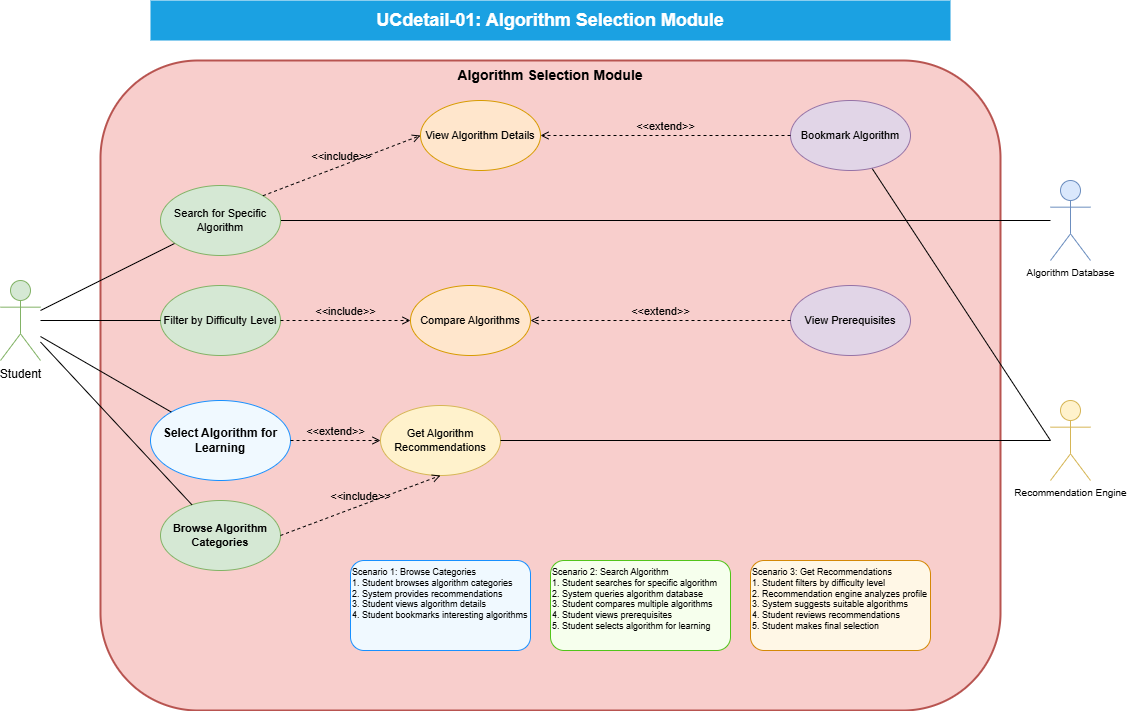
\includegraphics[width=1.0\textwidth]{enhanced-diagrams/UCdetail-01-algorithm-selection.png}
\caption{Use Case Diagram - System Overview}
\label{fig:usecase-system-overview}
\end{figure}

\subsection{Phân nhóm Use Case theo Chức năng}
\label{subsec:use-case-functional-groups}

Các use case được tổ chức thành 4 nhóm chức năng chính:

\subsubsection{Student Learning Group (5 use cases)}
\begin{enumerate}
    \item \textbf{Learn Algorithm Concepts}: Học các khái niệm thuật toán cơ bản
    \item \textbf{Practice with Visualizations}: Thực hành với animation tương tác
    \item \textbf{Take Assessments}: Thực hiện các bài kiểm tra đánh giá
    \item \textbf{Track Learning Progress}: Theo dõi tiến độ học tập cá nhân
    \item \textbf{Collaborate with Peers}: Tương tác và học tập cùng đồng học
\end{enumerate}

\subsubsection{Instructor Management Group (4 use cases)}
\begin{enumerate}
    \item \textbf{Manage Learning Content}: Quản lý nội dung học tập và tài liệu
    \item \textbf{Create Assessments}: Tạo các bài kiểm tra và quiz
    \item \textbf{Monitor Student Progress}: Theo dõi tiến độ học tập của học viên
    \item \textbf{Manage Classes}: Quản lý lớp học và nhóm học viên
\end{enumerate}

\subsubsection{System Administration Group (4 use cases)}
\begin{enumerate}
    \item \textbf{Manage System Users}: Quản lý tài khoản và quyền người dùng
    \item \textbf{System Maintenance}: Bảo trì và cập nhật hệ thống
    \item \textbf{Monitor System Performance}: Giám sát hiệu suất hệ thống
    \item \textbf{Security Management}: Quản lý bảo mật và quyền truy cập
\end{enumerate}

\subsubsection{Core System Support Group (5 use cases)}
\begin{enumerate}
    \item \textbf{User Authentication}: Xác thực và quản lý phiên đăng nhập
    \item \textbf{Data Management}: Quản lý dữ liệu và storage
    \item \textbf{AI-Powered Assistance}: Cung cấp hỗ trợ AI thông minh
    \item \textbf{Send Notifications}: Gửi thông báo và cảnh báo
    \item \textbf{Generate Analytics}: Tạo báo cáo và phân tích dữ liệu
\end{enumerate}

\subsection{Detailed Use Case Specifications}
\label{subsec:detailed-usecase-specs}

Phần này trình bày chi tiết các use case chính của hệ thống theo format chuẩn academic, mô tả đầy đủ các luồng sự kiện, điều kiện tiên quyết, và kết quả mong đợi.

\subsubsection{UC001: Algorithm Visualization Learning}

\begin{longtable}{| p{3cm} | p{10cm} |}
\hline
\textbf{Use Case ID} & UC001 \\ \hline
\textbf{Tên Use Case} & Algorithm Visualization Learning \\ \hline
\textbf{Actor} & Student \\ \hline
\textbf{Mô tả ngắn gọn} & Học viên học thuật toán thông qua visualization interactive \\ \hline
\textbf{Trigger} & Học viên muốn học và hiểu thuật toán thông qua visualization \\ \hline
\textbf{Precondition} & 
\begin{itemize}
    \item Học viên đã đăng nhập vào hệ thống
    \item Hệ thống có sẵn algorithm content
    \item Browser hỗ trợ HTML5 Canvas/WebGL
\end{itemize} \\ \hline
\textbf{Luồng sự kiện chính} & 
\begin{enumerate}
    \item Học viên chọn loại thuật toán muốn học
    \item Hệ thống hiển thị danh sách algorithms available
    \item Học viên chọn specific algorithm (VD: Quick Sort)
    \item Hệ thống load algorithm visualizer interface
    \item Học viên input dữ liệu hoặc sử dụng sample data
    \item Học viên bắt đầu visualization process
    \item Hệ thống thực hiện step-by-step animation
    \item Học viên control speed, pause, resume theo nhu cầu
    \item Hệ thống hiển thị complexity analysis và explanation
    \item Học viên hoàn thành learning session
\end{enumerate} \\ \hline
\textbf{Luồng sự kiện thay thế} & 
\textbf{Alt 1:} Học viên muốn compare algorithms
\begin{itemize}
    \item Từ bước 3, học viên chọn multiple algorithms
    \item Hệ thống hiển thị comparison view
    \item Học viên chạy cùng lúc để so sánh performance
\end{itemize} \\ \hline
\textbf{Luồng ngoại lệ} & 
\textbf{Exc 1:} Input data không hợp lệ
\begin{itemize}
    \item Hệ thống hiển thị error message
    \item Yêu cầu học viên nhập lại data
\end{itemize}
\textbf{Exc 2:} Algorithm execution error
\begin{itemize}
    \item Hệ thống reset visualization
    \item Hiển thị default sample data
\end{itemize} \\ \hline
\textbf{Post Condition} & 
\begin{itemize}
    \item Learning progress được cập nhật
    \item Session data được lưu trong profile
    \item Analytics data được ghi nhận
\end{itemize} \\ \hline
\caption{Use Case Scenario: Algorithm Visualization Learning}
\label{tab:uc001} \\
\end{longtable}

\subsubsection{UC002: Interactive Algorithm Practice}

\begin{longtable}{| p{3cm} | p{10cm} |}
\hline
\textbf{Use Case ID} & UC002 \\ \hline
\textbf{Tên Use Case} & Interactive Algorithm Practice \\ \hline
\textbf{Actor} & Student \\ \hline
\textbf{Mô tả ngắn gọn} & Học viên thực hành thuật toán với interactive controls và custom input để củng cố kiến thức \\ \hline
\textbf{Trigger} & Học viên muốn thực hành và kiểm tra hiểu biết về thuật toán đã học \\ \hline
\textbf{Precondition} & 
\begin{itemize}
    \item Học viên đã hoàn thành basic visualization learning
    \item Practice environment được kích hoạt
    \item Algorithm templates có sẵn trong hệ thống
\end{itemize} \\ \hline
\textbf{Luồng sự kiện chính} & 
\begin{enumerate}
    \item Học viên chọn "Practice Mode" từ algorithm interface
    \item Hệ thống hiển thị danh sách available practice algorithms
    \item Học viên chọn specific algorithm để practice
    \item Hệ thống load interactive practice environment với controls
    \item Học viên tạo custom input data hoặc chọn từ preset examples
    \item Học viên predict algorithm behavior trước khi execute
    \item Học viên execute algorithm với step-by-step controls
    \item Hệ thống provide real-time feedback và performance hints
    \item Học viên so sánh prediction với actual execution result
    \item Hệ thống calculate practice score và provide improvement suggestions
\end{enumerate} \\ \hline
\textbf{Luồng sự kiện thay thế} & 
\textbf{Alt 1:} Guided Practice Mode
\begin{itemize}
    \item Hệ thống cung cấp hints và step-by-step guidance
    \item Học viên được hỗ trợ với detailed explanations cho mỗi step
\end{itemize}
\textbf{Alt 2:} Challenge Practice Mode
\begin{itemize}
    \item Hệ thống đưa ra specific challenges với time constraints
    \item Học viên phải complete tasks trong giới hạn thời gian
\end{itemize} \\ \hline
\textbf{Luồng ngoại lệ} & 
\textbf{Exc 1:} Invalid practice input data
\begin{itemize}
    \item Hệ thống validate input và hiển thị specific error messages
    \item Provide suggested valid input examples và format guidelines
\end{itemize}
\textbf{Exc 2:} Practice session timeout
\begin{itemize}
    \item Hệ thống auto-save current progress và state
    \item Cho phép học viên resume từ saved checkpoint
\end{itemize} \\ \hline
\textbf{Post Condition} & 
\begin{itemize}
    \item Practice performance score được record vào user profile
    \item Skill assessment metrics được update dựa trên performance
    \item Achievement badges có thể được unlock
    \item Practice history được save cho future reference và review
\end{itemize} \\ \hline
\caption{Use Case Scenario: Interactive Algorithm Practice}
\label{tab:uc002} \\
\end{longtable}

\subsubsection{UC003: AI Assistant Consultation}

\begin{longtable}{| p{3cm} | p{10cm} |}
\hline
\textbf{Use Case ID} & UC003 \\ \hline
\textbf{Tên Use Case} & AI Assistant Consultation \\ \hline
\textbf{Actor} & Student \\ \hline
\textbf{Mô tả ngắn gọn} & Học viên tương tác với AI Assistant để nhận hỗ trợ học tập thông minh và giải đáp thắc mắc \\ \hline
\textbf{Trigger} & Học viên gặp khó khăn hoặc cần explanations chi tiết về algorithm concepts \\ \hline
\textbf{Precondition} & 
\begin{itemize}
    \item Học viên đang trong active learning session
    \item AI Assistant service đang available và responsive
    \item Network connection stable cho real-time interaction
    \item Current learning context được load successfully
\end{itemize} \\ \hline
\textbf{Luồng sự kiện chính} & 
\begin{enumerate}
    \item Học viên click vào AI Assistant icon trong learning interface
    \item Hệ thống mở AI chat interface với current context loading
    \item Học viên nhập câu hỏi về algorithm hiện tại hoặc related concepts
    \item AI Assistant analyze question context và intent recognition
    \item AI generate comprehensive response với examples và explanations
    \item Hệ thống display AI answer với proper formatting và code highlighting
    \item Học viên có thể ask follow-up questions để clarify doubts
    \item AI provide additional learning resources và hints nếu appropriate
    \item Học viên close AI Assistant khi satisfied với answers
    \item Hệ thống save conversation history cho future reference
\end{enumerate} \\ \hline
\textbf{Luồng sự kiện thay thế} & 
\textbf{Alt 1:} Code Analysis Request
\begin{itemize}
    \item Học viên paste existing code snippet để AI review
    \item AI analyze code quality và suggest optimizations với detailed explanations
\end{itemize}
\textbf{Alt 2:} Algorithm Recommendation
\begin{itemize}
    \item Học viên describe specific problem cần solve
    \item AI recommend suitable algorithms với pros/cons comparison
\end{itemize}
\textbf{Alt 3:} Step-by-step Explanation
\begin{itemize}
    \item Học viên request explanation cho current visualization step
    \item AI provide synchronized explanation với animation context
\end{itemize} \\ \hline
\textbf{Luồng ngoại lệ} & 
\textbf{Exc 1:} AI service temporarily unavailable
\begin{itemize}
    \item Hệ thống display fallback resources và static documentation
    \item Redirect đến FAQ hoặc community knowledge base
    \item Log incident cho service monitoring
\end{itemize}
\textbf{Exc 2:} Question too complex hoặc ambiguous
\begin{itemize}
    \item AI request clarification với specific guiding questions
    \item Suggest breaking down complex question thành smaller parts
\end{itemize}
\textbf{Exc 3:} Rate limiting exceeded
\begin{itemize}
    \item Display rate limit message với cooldown timer
    \item Suggest alternative help resources during waiting period
\end{itemize} \\ \hline
\textbf{Post Condition} & 
\begin{itemize}
    \item Conversation history được save trong user learning profile
    \item AI interaction data contribute đến model improvement
    \item User satisfaction feedback được collect tự động
    \item Related learning materials được suggest based on interaction patterns
    \item Learning analytics được update với AI usage metrics
\end{itemize} \\ \hline
\caption{Use Case Scenario: AI Assistant Consultation}
\label{tab:uc003} \\
\end{longtable}

\subsubsection{UC004: Algorithm Comparison Analysis}

\begin{longtable}{| p{3cm} | p{10cm} |}
\hline
\textbf{Use Case ID} & UC004 \\ \hline
\textbf{Tên Use Case} & Algorithm Comparison Analysis \\ \hline
\textbf{Actor} & Student \\ \hline
\textbf{Mô tả ngắn gọn} & Học viên so sánh performance và characteristics của multiple algorithms cùng lúc \\ \hline
\textbf{Trigger} & Học viên muốn hiểu sự khác biệt và trade-offs giữa các algorithms \\ \hline
\textbf{Precondition} & 
\begin{itemize}
    \item Ít nhất 2 algorithms được available cho comparison
    \item Comparison interface được support bởi browser
    \item Input data compatible với tất cả algorithms được chọn
\end{itemize} \\ \hline
\textbf{Luồng sự kiện chính} & 
\begin{enumerate}
    \item Học viên chọn "Compare Algorithms" từ algorithm library
    \item Hệ thống hiển thị selection interface cho multiple algorithms
    \item Học viên chọn 2-4 algorithms để compare (VD: Bubble Sort vs Quick Sort vs Merge Sort)
    \item Hệ thống load comparison interface với side-by-side views
    \item Học viên configure common input data cho all algorithms
    \item Học viên start simultaneous execution của tất cả algorithms
    \item Hệ thống run algorithms concurrently với synchronized visualization
    \item Display real-time performance metrics: time complexity, space usage, steps count
    \item Học viên có thể adjust execution speed và pause/resume all algorithms
    \item Hệ thống present final comparison results với statistical analysis
\end{enumerate} \\ \hline
\textbf{Luồng sự kiện thay thế} & 
\textbf{Alt 1:} Different Input Sizes Comparison
\begin{itemize}
    \item Học viên chọn multiple input sizes để test scalability
    \item Hệ thống run algorithms với different dataset sizes
    \item Display performance scaling charts và complexity analysis
\end{itemize}
\textbf{Alt 2:} Best/Worst Case Analysis
\begin{itemize}
    \item Học viên select specific test cases: best, average, worst case scenarios
    \item Hệ thống generate appropriate input data cho each scenario
\end{itemize} \\ \hline
\textbf{Luồng ngoại lệ} & 
\textbf{Exc 1:} Incompatible algorithm selection
\begin{itemize}
    \item Hệ thống detect algorithms không thể compare directly
    \item Suggest alternative algorithms hoặc provide explanation về incompatibility
\end{itemize}
\textbf{Exc 2:} Performance measurement error
\begin{itemize}
    \item Hệ thống retry measurement với adjusted parameters
    \item Provide approximate results với confidence intervals
\end{itemize} \\ \hline
\textbf{Post Condition} & 
\begin{itemize}
    \item Comparison results được save trong user learning history
    \item Performance benchmarks được contribute đến system analytics
    \item Understanding assessment được update based on comparison insights
    \item Related learning resources được suggest for deeper understanding
\end{itemize} \\ \hline
\caption{Use Case Scenario: Algorithm Comparison Analysis}
\label{tab:uc004} \\
\end{longtable}

\subsubsection{UC005: Learning Progress Tracking}

\begin{longtable}{| p{3cm} | p{10cm} |}
\hline
\textbf{Use Case ID} & UC005 \\ \hline
\textbf{Tên Use Case} & Learning Progress Tracking \\ \hline
\textbf{Actor} & Student \\ \hline
\textbf{Mô tả ngắn gọn} & Học viên theo dõi và review learning progress với detailed analytics và recommendations \\ \hline
\textbf{Trigger} & Học viên muốn review learning achievements và plan next learning steps \\ \hline
\textbf{Precondition} & 
\begin{itemize}
    \item Học viên đã có ít nhất một learning session được completed
    \item Progress tracking service đang hoạt động normally
    \item User profile data accessible và up-to-date
\end{itemize} \\ \hline
\textbf{Luồng sự kiện chính} & 
\begin{enumerate}
    \item Học viên access "My Progress" dashboard từ main navigation
    \item Hệ thống load comprehensive progress data và analytics
    \item Display overall learning statistics: algorithms completed, time spent, skill levels
    \item Show detailed breakdown theo algorithm categories và difficulty levels
    \item Present learning trajectory với progress over time charts
    \item Display achievement badges earned và milestones reached
    \item Show personalized recommendations cho next learning objectives
    \item Học viên có thể drill down vào specific algorithm performance details
    \item Review practice scores và assessment results với trend analysis
    \item Set learning goals và targets cho upcoming study sessions
\end{enumerate} \\ \hline
\textbf{Luồng sự kiện thay thế} & 
\textbf{Alt 1:} Comparison với Peer Performance
\begin{itemize}
    \item Học viên enable anonymous peer comparison features
    \item Hệ thống show relative performance metrics so với class/group averages
\end{itemize}
\textbf{Alt 2:} Detailed Time Analysis
\begin{itemize}
    \item Học viên request detailed time spending analysis
    \item Display time allocation across different learning activities
\end{itemize}
\textbf{Alt 3:} Export Progress Report
\begin{itemize}
    \item Học viên request downloadable progress report
    \item Hệ thống generate PDF report với comprehensive analytics
\end{itemize} \\ \hline
\textbf{Luồng ngoại lệ} & 
\textbf{Exc 1:} Insufficient progress data
\begin{itemize}
    \item Hệ thống notify về minimum data requirements
    \item Suggest completing more learning activities để unlock full analytics
\end{itemize}
\textbf{Exc 2:} Analytics service unavailable
\begin{itemize}
    \item Display cached progress data với timestamp indication
    \item Schedule automatic refresh khi service becomes available
\end{itemize} \\ \hline
\textbf{Post Condition} & 
\begin{itemize}
    \item Progress review activity được log cho usage analytics
    \item Learning goals và targets được save in user profile
    \item Recommendation engine được update với user interaction patterns
    \item Motivation metrics được calculate based on progress review frequency
\end{itemize} \\ \hline
\caption{Use Case Scenario: Learning Progress Tracking}
\label{tab:uc005} \\
\end{longtable}

\section{Class Diagram}
\label{sec:class-diagram}

\subsection{Tổng quan Class Diagram}
\label{subsec:class-overview}

Class diagram của hệ thống DSA Visualizer được thiết kế theo mô hình MVC (Model-View-Controller) và Clean Architecture, đảm bảo tính modular và scalability.

\begin{center}
\textbf{[Class Diagram - Core System]}\\
\textit{Diagram: class-diagram-clean.drawio}
\end{center}

\subsection{Các nhóm Class chính}

\subsubsection{User Management Classes}

\textbf{User Class:}
\begin{itemize}
    \item \textbf{Thuộc tính:} userID, email, username, password, role, createdAt, lastLogin
    \item \textbf{Phương thức:} login(), logout(), updateProfile(), changePassword()
    \item \textbf{Mối quan hệ:} User có nhiều LearningSession, có một UserProfile
\end{itemize}

\textbf{UserProfile Class:}
\begin{itemize}
    \item \textbf{Thuộc tính:} profileID, firstName, lastName, avatar, bio, preferences
    \item \textbf{Phương thức:} updatePersonalInfo(), setPreferences(), uploadAvatar()
    \item \textbf{Mối quan hệ:} Thuộc về một User, có nhiều Achievement
\end{itemize}

\subsubsection{Algorithm Visualization Classes}

\textbf{Algorithm Class:}
\begin{itemize}
    \item \textbf{Thuộc tính:} algorithmID, name, category, description, complexity, difficulty
    \item \textbf{Phương thức:} execute(), visualize(), getComplexity(), generateSteps()
    \item \textbf{Mối quan hệ:} Có nhiều AlgorithmStep, thuộc về một Category
\end{itemize}

\textbf{Visualizer Class:}
\begin{itemize}
    \item \textbf{Thuộc tính:} visualizerID, type, config, animationSpeed, currentStep
    \item \textbf{Phương thức:} start(), pause(), resume(), reset(), setSpeed()
    \item \textbf{Mối quan hệ:} Sử dụng Algorithm, tạo ra VisualizationSession
\end{itemize}

\textbf{AlgorithmStep Class:}
\begin{itemize}
    \item \textbf{Thuộc tính:} stepID, stepNumber, description, dataState, action
    \item \textbf{Phương thức:} execute(), undo(), getDescription(), visualize()
    \item \textbf{Mối quan hệ:} Thuộc về một Algorithm
\end{itemize}

\subsubsection{Learning Management Classes}

\textbf{LearningSession Class:}
\begin{itemize}
    \item \textbf{Thuộc tính:} sessionID, userID, algorithmID, startTime, endTime, score
    \item \textbf{Phương thức:} start(), complete(), calculateScore(), saveProgress()
    \item \textbf{Mối quan hệ:} Thuộc về User và Algorithm
\end{itemize}

\textbf{Progress Class:}
\begin{itemize}
    \item \textbf{Thuộc tính:} progressID, userID, totalSessions, completedAlgorithms, skillLevel
    \item \textbf{Phương thức:} updateProgress(), calculateSkillLevel(), getStatistics()
    \item \textbf{Mối quan hệ:} Thuộc về một User
\end{itemize}

\subsubsection{Assessment Classes}

\textbf{Quiz Class:}
\begin{itemize}
    \item \textbf{Thuộc tính:} quizID, title, description, questions, timeLimit, difficulty
    \item \textbf{Phương thức:} generateQuestions(), calculateScore(), validateAnswers()
    \item \textbf{Mối quan hệ:} Có nhiều Question, có nhiều QuizResult
\end{itemize}

\textbf{Question Class:}
\begin{itemize}
    \item \textbf{Thuộc tính:} questionID, content, options, correctAnswer, explanation
    \item \textbf{Phương thức:} validateAnswer(), getHint(), getExplanation()
    \item \textbf{Mối quan hệ:} Thuộc về một Quiz
\end{itemize}

\subsection{Design Patterns được sử dụng}

\subsubsection{Factory Pattern}
Sử dụng AlgorithmFactory để tạo ra các instance của different algorithm types:
\begin{itemize}
    \item SortingAlgorithmFactory
    \item SearchAlgorithmFactory  
    \item GraphAlgorithmFactory
\end{itemize}

\subsubsection{Observer Pattern}
VisualizationObserver được implement để notify UI components khi algorithm state changes:
\begin{itemize}
    \item ProgressObserver: Cập nhật progress bar
    \item AnimationObserver: Trigger animation effects
    \item ScoreObserver: Calculate và display scores
\end{itemize}

\subsubsection{Strategy Pattern}
Sử dụng cho algorithm execution strategies:
\begin{itemize}
    \item StepByStepStrategy: Execute từng bước
    \item ContinuousStrategy: Execute liên tục
    \item ComparisonStrategy: So sánh multiple algorithms
\end{itemize}

\section{Activity Diagram}
\label{sec:activity-diagram}

\subsection{Tổng quan Activity Diagram}
\label{subsec:activity-overview}

Activity diagram mô tả luồng hoạt động chính của hệ thống, từ khi user đăng nhập cho đến khi hoàn thành learning session.

\begin{center}
\textbf{[Activity Diagram - Learning Process]}\\
\textit{Diagram: activity-diagram-clean.drawio}
\end{center}

\subsection{Quy trình hoạt động chính}

\subsubsection{Authentication Flow}
\begin{enumerate}
    \item \textbf{Start:} User truy cập application
    \item \textbf{Decision:} Kiểm tra user đã login chưa?
    \item \textbf{False:} Redirect đến login page
    \item \textbf{Login Process:} User nhập credentials
    \item \textbf{Validation:} System validate user information
    \item \textbf{Decision:} Credentials có hợp lệ?
    \item \textbf{False:} Show error message, return to login
    \item \textbf{True:} Generate JWT token, redirect to dashboard
\end{enumerate}

\subsubsection{Algorithm Learning Flow}
\begin{enumerate}
    \item \textbf{Dashboard Access:} User vào main dashboard
    \item \textbf{Category Selection:} User chọn algorithm category
    \item \textbf{Algorithm Selection:} User chọn specific algorithm
    \item \textbf{Visualizer Loading:} System load algorithm visualizer
    \item \textbf{Input Configuration:} User configure input data
    \item \textbf{Decision:} User muốn start visualization?
    \item \textbf{True:} Begin algorithm execution
    \item \textbf{Step-by-step Execution:} System execute từng step
    \item \textbf{Animation Rendering:} Display visual animation
    \item \textbf{User Interaction:} User có thể pause/resume/adjust speed
    \item \textbf{Completion Check:} Algorithm execution complete?
    \item \textbf{False:} Continue next step
    \item \textbf{True:} Display final result và complexity analysis
\end{enumerate}

\subsubsection{AI Assistant Flow}
\begin{enumerate}
    \item \textbf{Trigger:} User click AI Assistant button
    \item \textbf{Context Collection:} System collect current learning context
    \item \textbf{Question Input:} User nhập question
    \item \textbf{NLP Processing:} AI analyze question intent
    \item \textbf{Knowledge Retrieval:} AI search relevant information
    \item \textbf{Response Generation:} AI generate appropriate response
    \item \textbf{Response Display:} System show AI response
    \item \textbf{Decision:} User có additional questions?
    \item \textbf{True:} Return to question input
    \item \textbf{False:} Close AI Assistant
\end{enumerate}

\subsubsection{Assessment Flow}
\begin{enumerate}
    \item \textbf{Quiz Selection:} User chọn quiz để làm
    \item \textbf{Quiz Loading:} System load quiz questions
    \item \textbf{Question Display:} Show current question
    \item \textbf{Answer Input:} User select/input answer
    \item \textbf{Answer Validation:} System validate answer
    \item \textbf{Feedback Display:} Show immediate feedback
    \item \textbf{Progress Update:} Update quiz progress
    \item \textbf{Decision:} Còn questions nào không?
    \item \textbf{True:} Next question
    \item \textbf{False:} Calculate final score
    \item \textbf{Result Display:} Show quiz results và recommendations
    \item \textbf{Progress Save:} Save user progress và achievements
\end{enumerate}

\subsection{Parallel Activities}

Hệ thống hỗ trợ các parallel activities:

\subsubsection{Background Services}
\begin{itemize}
    \item \textbf{Analytics Collection:} Continuous tracking user behavior
    \item \textbf{Performance Monitoring:} Real-time system performance tracking
    \item \textbf{Cache Management:} Background cache invalidation và refresh
    \item \textbf{Notification Processing:} Async notification sending
\end{itemize}

\subsubsection{Real-time Features}
\begin{itemize}
    \item \textbf{Live Progress Updates:} Real-time progress synchronization
    \item \textbf{Community Activity:} Live discussion forum updates
    \item \textbf{Collaborative Learning:} Multi-user learning sessions
\end{itemize}

\section{Sequence Diagram}
\label{sec:sequence-diagram}

\subsection{Tổng quan Sequence Diagram}
\label{subsec:sequence-overview}

Sequence diagram minh họa tương tác giữa các objects trong hệ thống theo thời gian, đặc biệt tập trung vào main learning scenarios.

\begin{center}
\textbf{[Sequence Diagram - Algorithm Learning Process]}\\
\textit{Diagram: sequence-diagram-clean.drawio}
\end{center}

\subsection{Chi tiết Sequence Interactions}

\subsubsection{Algorithm Visualization Sequence}

\textbf{Actors/Objects tham gia:}
\begin{itemize}
    \item Student (Actor)
    \item UI Controller
    \item Algorithm Service
    \item Visualizer Engine
    \item Database
    \item AI Assistant Service
\end{itemize}

\textbf{Sequence of Messages:}

\begin{enumerate}
    \item \textbf{Student → UI Controller:} selectAlgorithm(algorithmType)
    \item \textbf{UI Controller → Algorithm Service:} loadAlgorithm(algorithmType)
    \item \textbf{Algorithm Service → Database:} getAlgorithmDetails(algorithmType)
    \item \textbf{Database → Algorithm Service:} algorithmDetails
    \item \textbf{Algorithm Service → UI Controller:} algorithmLoaded
    \item \textbf{UI Controller → Student:} displayAlgorithmInterface()
    \item \textbf{Student → UI Controller:} configureInput(inputData)
    \item \textbf{UI Controller → Algorithm Service:} validateInput(inputData)
    \item \textbf{Algorithm Service → UI Controller:} inputValid
    \item \textbf{Student → UI Controller:} startVisualization()
    \item \textbf{UI Controller → Visualizer Engine:} initializeVisualization(algorithm, data)
    \item \textbf{Visualizer Engine → Algorithm Service:} executeStep()
    \item \textbf{Algorithm Service → Visualizer Engine:} stepResult
    \item \textbf{Visualizer Engine → UI Controller:} updateVisualization(stepResult)
    \item \textbf{UI Controller → Student:} displayAnimation()
    \item \textbf{Loop:} Repeat steps 12-15 until completion
    \item \textbf{Visualizer Engine → UI Controller:} visualizationComplete()
    \item \textbf{UI Controller → Database:} saveProgress(userId, sessionData)
    \item \textbf{UI Controller → Student:} displayResults(finalState, complexity)
\end{enumerate}

\subsubsection{AI Assistant Interaction Sequence}

\textbf{Sequence of Messages:}

\begin{enumerate}
    \item \textbf{Student → UI Controller:} openAIAssistant()
    \item \textbf{UI Controller → AI Assistant Service:} initializeSession(userId, context)
    \item \textbf{AI Assistant Service → Database:} getUserLearningContext(userId)
    \item \textbf{Database → AI Assistant Service:} learningContext
    \item \textbf{AI Assistant Service → UI Controller:} sessionReady
    \item \textbf{UI Controller → Student:} displayChatInterface()
    \item \textbf{Student → UI Controller:} askQuestion(question)
    \item \textbf{UI Controller → AI Assistant Service:} processQuestion(question, context)
    \item \textbf{AI Assistant Service:} analyzeIntent(question)
    \item \textbf{AI Assistant Service:} retrieveKnowledge(intent)
    \item \textbf{AI Assistant Service:} generateResponse(knowledge, context)
    \item \textbf{AI Assistant Service → UI Controller:} response
    \item \textbf{UI Controller → Student:} displayResponse(response)
    \item \textbf{AI Assistant Service → Database:} logInteraction(userId, question, response)
\end{enumerate}

\subsubsection{Assessment and Quiz Sequence}

\textbf{Sequence of Messages:}

\begin{enumerate}
    \item \textbf{Student → UI Controller:} selectQuiz(quizId)
    \item \textbf{UI Controller → Assessment Service:} loadQuiz(quizId)
    \item \textbf{Assessment Service → Database:} getQuizDetails(quizId)
    \item \textbf{Database → Assessment Service:} quizData
    \item \textbf{Assessment Service → UI Controller:} quizLoaded
    \item \textbf{UI Controller → Student:} displayQuizInterface()
    \item \textbf{Student → UI Controller:} startQuiz()
    \item \textbf{UI Controller → Assessment Service:} beginQuizSession(userId, quizId)
    \item \textbf{Loop for each question:}
    \begin{enumerate}
        \item \textbf{Assessment Service → UI Controller:} getNextQuestion()
        \item \textbf{UI Controller → Student:} displayQuestion(question)
        \item \textbf{Student → UI Controller:} submitAnswer(answer)
        \item \textbf{UI Controller → Assessment Service:} validateAnswer(questionId, answer)
        \item \textbf{Assessment Service → UI Controller:} answerResult(correct, explanation)
        \item \textbf{UI Controller → Student:} showFeedback(result, explanation)
    \end{enumerate}
    \item \textbf{Assessment Service → UI Controller:} calculateFinalScore()
    \item \textbf{UI Controller → Database:} saveQuizResult(userId, quizId, score, answers)
    \item \textbf{UI Controller → Student:} displayFinalResults(score, recommendations)
\end{enumerate}

\subsection{Error Handling Sequences}

\subsubsection{Authentication Error Sequence}
\begin{enumerate}
    \item \textbf{Student → UI Controller:} login(credentials)
    \item \textbf{UI Controller → Auth Service:} validateCredentials(credentials)
    \item \textbf{Auth Service → Database:} checkUserCredentials(credentials)
    \item \textbf{Database → Auth Service:} userNotFound/invalidPassword
    \item \textbf{Auth Service → UI Controller:} authenticationFailed(errorType)
    \item \textbf{UI Controller → Student:} displayErrorMessage(errorType)
    \item \textbf{UI Controller → Student:} requestCredentialsAgain()
\end{enumerate}

\subsubsection{System Error Recovery Sequence}
\begin{enumerate}
    \item \textbf{Any Service:} systemError(errorDetails)
    \item \textbf{Error Handler:} logError(errorDetails)
    \item \textbf{Error Handler → Monitoring Service:} reportError(errorDetails)
    \item \textbf{Error Handler → UI Controller:} notifyUser(genericErrorMessage)
    \item \textbf{UI Controller → Student:} displayErrorScreen(recoveryOptions)
    \item \textbf{Error Handler:} attemptRecovery()
    \item \textbf{Fallback Service:} provideFallbackFunctionality()
\end{enumerate}

\section{System Architecture Analysis}
\label{sec:system-architecture}

\subsection{Tổng quan Architecture}
\label{subsec:architecture-overview}

Hệ thống DSA Visualizer được thiết kế theo mô hình 5-layer architecture để đảm bảo scalability, maintainability và performance optimization.

\begin{center}
\textbf{[System Architecture Diagram]}\\
\textit{Diagram: system-architecture.drawio}
\end{center}

\subsection{Chi tiết các Layer}

\subsubsection{UI Layer (Presentation Layer)}
\textbf{Công nghệ sử dụng:} Next.js 14, React 18, TypeScript, TailwindCSS

\textbf{Thành phần chính:}
\begin{itemize}
    \item \textbf{Interactive Visualizers:} Canvas-based algorithm animations
    \item \textbf{Control Panels:} Speed control, step-by-step navigation
    \item \textbf{Dashboard Interface:} User progress tracking và statistics
    \item \textbf{AI Chat Interface:} Real-time chat với AI Assistant
    \item \textbf{Assessment Interface:} Quiz và practice exercises
\end{itemize}

\textbf{Design Patterns:}
\begin{itemize}
    \item Component-based architecture
    \item State management với Context API
    \item Custom hooks cho reusable logic
    \item Responsive design patterns
\end{itemize}

\subsubsection{Visualization Engine Layer}
\textbf{Công nghệ sử dụng:} D3.js, Canvas API, WebGL

\textbf{Core Components:}
\begin{itemize}
    \item \textbf{Animation Controller:} Quản lý animation timeline và state
    \item \textbf{Rendering Engine:} High-performance visualization rendering
    \item \textbf{Interaction Handler:} User input processing cho visualizations
    \item \textbf{State Manager:} Algorithm state tracking và history
\end{itemize}

\textbf{Visualization Types:}
\begin{itemize}
    \item Array/List visualizations với color coding
    \item Tree structures với interactive nodes
    \item Graph visualizations với edge animations
    \item Comparison views cho multiple algorithms
\end{itemize}

\subsubsection{Backend Services Layer}
\textbf{Công nghệ sử dụng:} Node.js, Express.js, TypeScript

\textbf{Microservices Architecture:}
\begin{itemize}
    \item \textbf{Algorithm Service:} Algorithm execution và step generation
    \item \textbf{User Service:} Authentication, profile management
    \item \textbf{Learning Service:} Progress tracking, session management
    \item \textbf{Assessment Service:} Quiz generation, scoring system
    \item \textbf{AI Service:} Natural language processing, knowledge retrieval
    \item \textbf{Analytics Service:} User behavior tracking, performance metrics
\end{itemize}

\textbf{API Design:}
\begin{itemize}
    \item RESTful APIs với OpenAPI documentation
    \item GraphQL endpoints cho complex data queries
    \item WebSocket connections cho real-time features
    \item Rate limiting và security middleware
\end{itemize}

\subsubsection{Data Management Layer}
\textbf{Công nghệ sử dụng:} MongoDB, Redis, PostgreSQL

\textbf{Database Strategy:}
\begin{itemize}
    \item \textbf{MongoDB:} User profiles, learning sessions, algorithm metadata
    \item \textbf{PostgreSQL:} Structured data, analytics, reporting
    \item \textbf{Redis:} Session caching, real-time data, leaderboards
\end{itemize}

\textbf{Data Models:}
\begin{itemize}
    \item User và Profile entities với relationship mapping
    \item Algorithm metadata với complexity analysis
    \item Learning progress với detailed tracking
    \item Assessment results với statistical analysis
\end{itemize}

\subsubsection{Infrastructure Layer}
\textbf{Deployment Strategy:} Docker containers, Kubernetes orchestration

\textbf{Cloud Services:}
\begin{itemize}
    \item \textbf{Compute:} Auto-scaling web servers
    \item \textbf{Storage:} Distributed file storage cho assets
    \item \textbf{CDN:} Global content delivery network
    \item \textbf{Monitoring:} Application performance monitoring
\end{itemize}

\textbf{Security Measures:}
\begin{itemize}
    \item JWT-based authentication với refresh tokens
    \item HTTPS enforcement với SSL certificates
    \item Input validation và SQL injection prevention
    \item Cross-Origin Resource Sharing (CORS) configuration
\end{itemize}

\subsection{Integration Patterns}

\subsubsection{Event-Driven Architecture}
\begin{itemize}
    \item User action events trigger visualization updates
    \item Progress events update learning analytics
    \item Achievement events trigger notification system
    \item Error events activate monitoring và alerting
\end{itemize}

\subsubsection{Caching Strategy}
\begin{itemize}
    \item Browser caching cho static assets
    \item Redis caching cho frequently accessed data
    \item CDN caching cho global performance
    \item Application-level caching cho computed results
\end{itemize}

\section{Design Principles và Best Practices}
\label{sec:design-principles}

\subsection{SOLID Principles Implementation}

\subsubsection{Single Responsibility Principle}
Mỗi class và component có một responsibility duy nhất:
\begin{itemize}
    \item VisualizationRenderer chỉ handle rendering logic
    \item AlgorithmExecutor chỉ handle algorithm execution
    \item UserManager chỉ handle user-related operations
\end{itemize}

\subsubsection{Open/Closed Principle}
Hệ thống được thiết kế để extend functionality without modification:
\begin{itemize}
    \item Plugin architecture cho new algorithm types
    \item Extension system cho custom visualizations
    \item Configurable assessment frameworks
\end{itemize}

\subsubsection{Liskov Substitution Principle}
Abstract classes và interfaces đảm bảo substitutability:
\begin{itemize}
    \item Algorithm interface có thể được implement bởi any algorithm type
    \item Visualizer interface support multiple rendering strategies
    \item Assessment interface accommodate different quiz types
\end{itemize}

\subsection{Performance Optimization}

\subsubsection{Frontend Optimization}
\begin{itemize}
    \item Code splitting và lazy loading cho components
    \item Memoization cho expensive computations
    \item Virtual scrolling cho large datasets
    \item Debouncing cho user input handling
\end{itemize}

\subsubsection{Backend Optimization}
\begin{itemize}
    \item Database query optimization với proper indexing
    \item Connection pooling cho database connections
    \item Asynchronous processing cho time-consuming tasks
    \item Load balancing cho high availability
\end{itemize}

\subsection{Accessibility và Usability}

\subsubsection{Accessibility Features}
\begin{itemize}
    \item WCAG 2.1 compliance cho accessibility standards
    \item Keyboard navigation support
    \item Screen reader compatibility
    \item High contrast mode cho visual impairments
\end{itemize}

\subsubsection{Usability Features}
\begin{itemize}
    \item Intuitive user interface design
    \item Progressive disclosure của complex features
    \item Contextual help và tooltips
    \item Responsive design cho multiple devices
\end{itemize}

\section{Kết luận Chapter 3}
\label{sec:chapter3-conclusion}

Chapter 3 đã phân tích chi tiết hệ thống DSA Visualizer từ góc độ technical architecture và design. Các điểm chính bao gồm:

\subsection{Use Case Analysis}
Đã định nghĩa và mô tả chi tiết các use cases chính của hệ thống, bao gồm algorithm learning, interactive practice, và AI assistant consultation. Mỗi use case được documented với format table chi tiết theo chuẩn academic.

\subsection{UML Diagrams Analysis}
\begin{itemize}
    \item \textbf{Class Diagram:} Thiết kế OOP với các design patterns phù hợp
    \item \textbf{Activity Diagram:} Mô tả chi tiết quy trình hoạt động và decision flows
    \item \textbf{Sequence Diagram:} Phân tích tương tác giữa objects theo timeline
\end{itemize}

\subsection{System Architecture}
Thiết kế 5-layer architecture đảm bảo:
\begin{itemize}
    \item Scalability cho future expansion
    \item Maintainability với modular design
    \item Performance optimization với caching strategies
    \item Security với comprehensive protection measures
\end{itemize}

\subsection{Technical Excellence}
Áp dụng SOLID principles, design patterns, và best practices để tạo ra một hệ thống robust và professional.

Tiếp theo, Chapter 4 sẽ focus vào implementation details và technical specifications của từng component.

\subsubsection{Use Case: Get AI Assistance}

\begin{longtable}{| p{3cm} | p{10cm} |}
\hline
\textbf{Use Case ID} & UC-AI-001 \\ \hline
\textbf{Tên Use Case} & Get AI Assistance \\ \hline
\textbf{Actor} & Student \\ \hline
\textbf{Mô tả ngắn gọn} & Student nhận hỗ trợ từ AI assistant để hiểu thuật toán hoặc giải quyết vấn đề \\ \hline
\textbf{Trigger} & Student gặp khó khăn và cần hỗ trợ trong quá trình học \\ \hline
\textbf{Precondition} & 
\begin{itemize}
    \item Student đã đăng nhập vào hệ thống
    \item AI service available và responsive
    \item Current learning context được load
\end{itemize} \\ \hline
\textbf{Luồng sự kiện chính} & 
\begin{enumerate}
    \item Student click "AI Assistant" button trong interface
    \item System mở AI chat interface với context loading
    \item Student nhập câu hỏi hoặc chọn suggested questions
    \item System gửi request đến AI service kèm theo context
    \item AI service process request và trả về comprehensive response
    \item System hiển thị AI response với proper formatting
    \item Student có thể tiếp tục conversation với follow-up questions
    \item System tự động lưu conversation history
\end{enumerate} \\ \hline
\textbf{Luồng sự kiện thay thế} & 
\textbf{Alt 1:} Code Generation Request
\begin{itemize}
    \item Student request code implementation cho current algorithm
    \item Student chọn programming language preference
    \item AI generate syntax-highlighted code với detailed explanation
\end{itemize}
\textbf{Alt 2:} Step-by-step Explanation
\begin{itemize}
    \item Student click "Explain Current Step" trong visualization
    \item AI explain current step synchronized với animation
\end{itemize} \\ \hline
\textbf{Luồng ngoại lệ} & 
\textbf{Exc 1:} AI Service Unavailable
\begin{itemize}
    \item AI service timeout hoặc connection error
    \item System show fallback static help resources
    \item Log error cho admin notification
\end{itemize}
\textbf{Exc 2:} Rate Limit Exceeded
\begin{itemize}
    \item Too many requests từ user trong short period
    \item System show rate limit message với countdown
    \item Suggest alternative help resources
\end{itemize} \\ \hline
\textbf{Post Condition} & 
\begin{itemize}
    \item Conversation history được lưu trong user profile
    \item AI usage statistics được cập nhật cho analytics
    \item Learning context được enrich từ conversation
    \item User satisfaction metrics được collect
\end{itemize} \\ \hline
\caption{Use Case Scenario: Get AI Assistance}
\label{tab:uc-ai-assistance} \\
\end{longtable}

\section{Class Diagram và Thiết kế Hướng đối tượng}
\label{sec:class-diagram}

\subsection{Tổng quan Class Diagram}
\label{subsec:class-overview}

Class diagram của hệ thống DSA Visualizer được thiết kế theo mô hình Clean Architecture và Domain-Driven Design, đảm bảo tính modular, scalability và maintainability. Hệ thống được tổ chức thành các layers rõ ràng với separation of concerns và loose coupling giữa các components.

\begin{figure}[H]
\centering
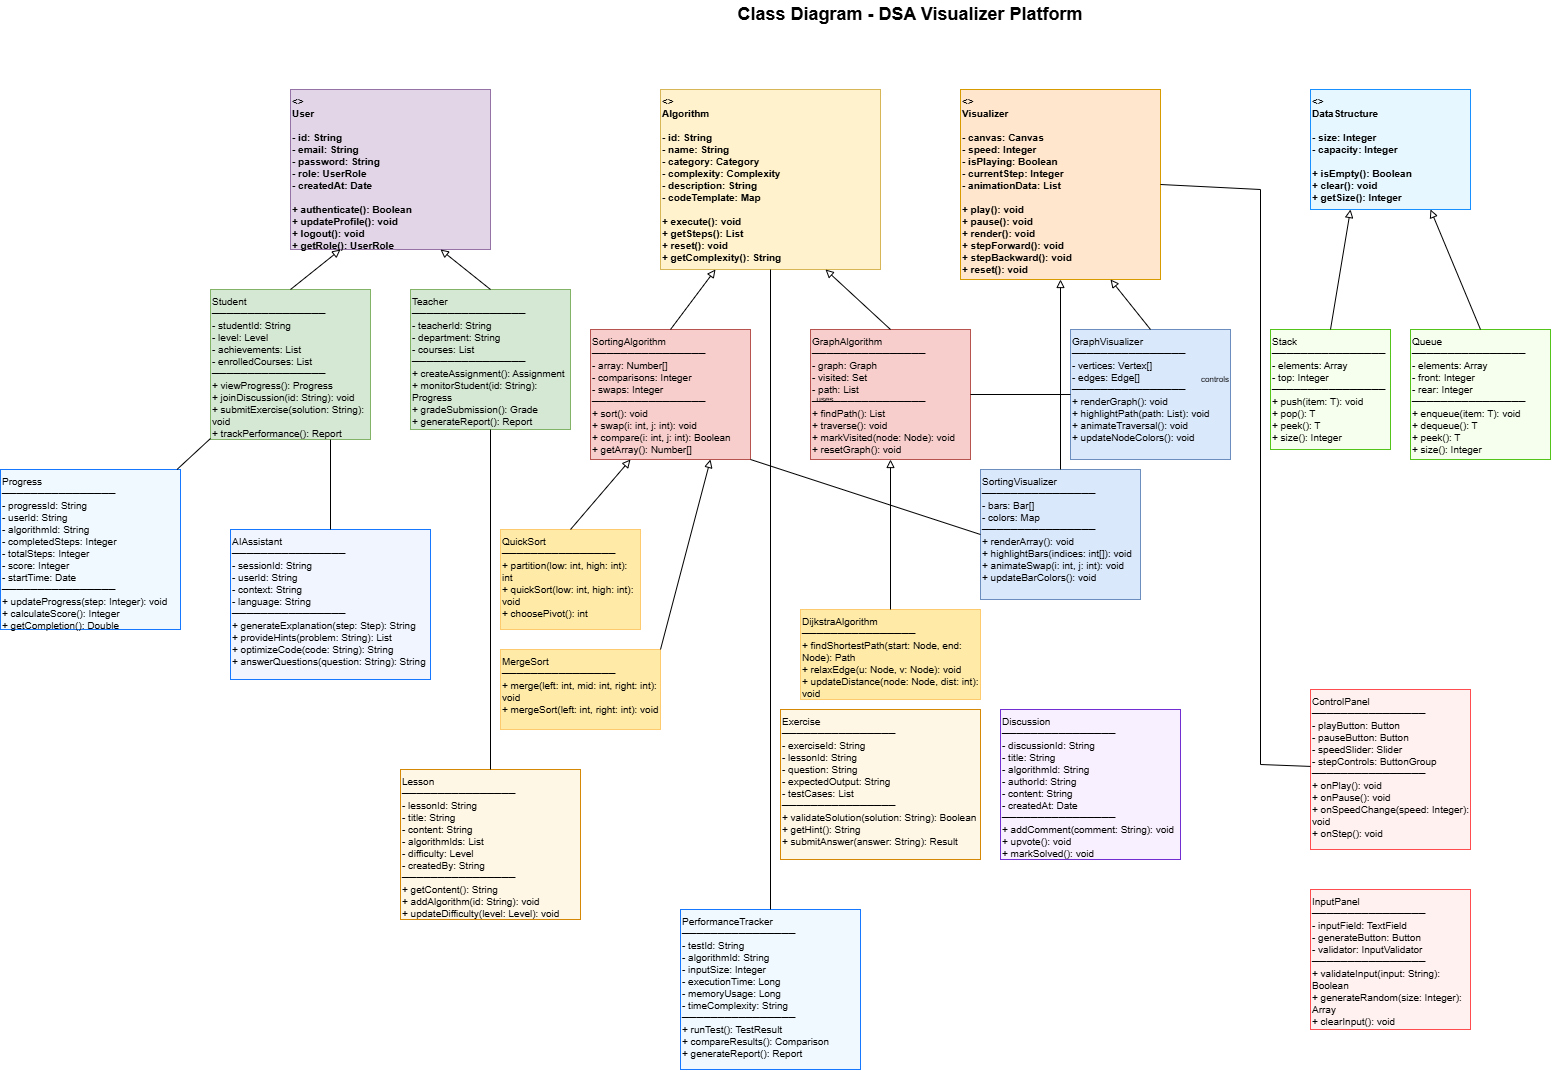
\includegraphics[width=1.0\textwidth]{enhanced-diagrams/class-diagram-clean.png}
\caption{Class Diagram - Core System Architecture}
\label{fig:class-diagram-overview}
\end{figure}

\subsection{Phân tích các Domain Classes}
\label{subsec:domain-classes}

\subsubsection{User Management Domain}

\textbf{User Abstract Class:}
\begin{itemize}
    \item \textbf{Attributes:} userID: String, email: String, username: String, password: String, role: UserRole, createdAt: DateTime, lastLogin: DateTime, isActive: Boolean
    \item \textbf{Methods:} login(): AuthResult, logout(): void, updateProfile(profile: UserProfile): void, changePassword(oldPass: String, newPass: String): Boolean
    \item \textbf{Relationships:} Abstract class được inherit bởi Student, Instructor, Administrator
\end{itemize}

\textbf{Student Class (extends User):}
\begin{itemize}
    \item \textbf{Additional Attributes:} studentID: String, currentLevel: SkillLevel, enrollmentDate: DateTime, preferredLanguage: String
    \item \textbf{Methods:} startLearningSession(algorithm: Algorithm): LearningSession, takeAssessment(quiz: Quiz): QuizResult, getProgress(): Progress
    \item \textbf{Relationships:} Has nhiều LearningSession, owns một Progress, participates trong nhiều Assessment
\end{itemize}

\textbf{Instructor Class (extends User):}
\begin{itemize}
    \item \textbf{Additional Attributes:} instructorID: String, department: String, specialization: String[], courses: Course[]
    \item \textbf{Methods:} createContent(content: LearningContent): void, createAssessment(quiz: Quiz): void, monitorStudents(classID: String): StudentProgress[]
    \item \textbf{Relationships:} Manages nhiều Course, creates nhiều LearningContent và Assessment
\end{itemize}

\subsubsection{Algorithm Visualization Domain}

\textbf{Algorithm Abstract Class:}
\begin{itemize}
    \item \textbf{Attributes:} algorithmID: String, name: String, category: AlgorithmCategory, description: String, timeComplexity: ComplexityInfo, spaceComplexity: ComplexityInfo, difficulty: DifficultyLevel
    \item \textbf{Methods:} execute(input: InputData): ExecutionResult, generateSteps(input: InputData): AlgorithmStep[], getComplexityAnalysis(): ComplexityAnalysis
    \item \textbf{Relationships:} Has nhiều AlgorithmStep, belongs to một Category, used in nhiều Visualization
\end{itemize}

\textbf{SortingAlgorithm Class (extends Algorithm):}
\begin{itemize}
    \item \textbf{Additional Attributes:} comparisonCount: Integer, swapCount: Integer, isStable: Boolean, isInPlace: Boolean
    \item \textbf{Methods:} sort(array: Array): SortedResult, compare(a: Element, b: Element): Integer, swap(i: Integer, j: Integer): void
    \item \textbf{Implementations:} BubbleSort, QuickSort, MergeSort, HeapSort classes
\end{itemize}

\textbf{VisualizationEngine Class:}
\begin{itemize}
    \item \textbf{Attributes:} engineID: String, renderingMode: RenderMode, animationSpeed: Float, currentStep: Integer, isPlaying: Boolean
    \item \textbf{Methods:} initialize(algorithm: Algorithm, data: InputData): void, start(): void, pause(): void, resume(): void, step(): void, reset(): void
    \item \textbf{Relationships:} Uses Algorithm, creates VisualizationSession, manages AnimationController
\end{itemize}

\subsubsection{Learning Management Domain}

\textbf{LearningSession Class:}
\begin{itemize}
    \item \textbf{Attributes:} sessionID: String, userID: String, algorithmID: String, startTime: DateTime, endTime: DateTime, duration: TimeSpan, completionStatus: SessionStatus
    \item \textbf{Methods:} start(): void, complete(): SessionResult, pause(): void, resume(): void, calculateScore(): Float, saveProgress(): void
    \item \textbf{Relationships:} Belongs to User và Algorithm, generates Progress updates
\end{itemize}

\textbf{Progress Class:}
\begin{itemize}
    \item \textbf{Attributes:} progressID: String, userID: String, totalSessions: Integer, completedAlgorithms: String[], skillLevel: SkillLevel, experiencePoints: Integer
    \item \textbf{Methods:} updateProgress(session: LearningSession): void, calculateSkillLevel(): SkillLevel, getStatistics(): ProgressStats, generateReport(): ProgressReport
    \item \textbf{Relationships:} Belongs to User, tracks multiple LearningSession
\end{itemize}

\subsubsection{Assessment và AI Support Domain}

\textbf{Quiz Class:}
\begin{itemize}
    \item \textbf{Attributes:} quizID: String, title: String, description: String, questions: Question[], timeLimit: Integer, passingScore: Float
    \item \textbf{Methods:} generateQuestions(algorithm: Algorithm): Question[], validateAnswers(answers: Answer[]): QuizResult, calculateScore(result: QuizResult): Float
    \item \textbf{Relationships:} Contains nhiều Question, generates nhiều QuizResult
\end{itemize}

\textbf{AIAssistant Class:}
\begin{itemize}
    \item \textbf{Attributes:} assistantID: String, modelType: AIModel, contextWindow: Integer, conversationHistory: Message[]
    \item \textbf{Methods:} processQuery(query: String, context: LearningContext): AIResponse, generateExplanation(algorithm: Algorithm): String, analyzeCode(code: String): CodeAnalysis
    \item \textbf{Relationships:} Supports LearningSession, generates AIResponse objects
\end{itemize}

\subsection{Service Layer Classes}
\label{subsec:service-classes}

\subsubsection{Visualization Services}

\textbf{VisualizationService Class:}
\begin{itemize}
    \item \textbf{Attributes:} serviceID: String, supportedAlgorithms: AlgorithmType[], renderingEngine: RenderingEngine
    \item \textbf{Methods:} createVisualization(algorithm: Algorithm, config: VisualizationConfig): Visualization, updateVisualization(step: AlgorithmStep): void
    \item \textbf{Design Patterns:} Implements Factory Pattern để tạo different visualization types
\end{itemize}

\textbf{AnimationController Class:}
\begin{itemize}
    \item \textbf{Attributes:} controllerID: String, frameRate: Integer, duration: Float, easingFunction: EasingType
    \item \textbf{Methods:} animateStep(step: AlgorithmStep): Animation, setSpeed(speed: Float): void, addKeyframe(keyframe: Keyframe): void
    \item \textbf{Design Patterns:} Observer Pattern để notify UI components về animation state changes
\end{itemize}

\subsubsection{AI Integration Services}

\textbf{AIServiceManager Class:}
\begin{itemize}
    \item \textbf{Attributes:} managerID: String, availableModels: AIModel[], currentModel: AIModel, rateLimiter: RateLimiter
    \item \textbf{Methods:} selectOptimalModel(queryType: QueryType): AIModel, processRequest(request: AIRequest): AIResponse, handleFallback(): FallbackResponse
    \item \textbf{Design Patterns:} Strategy Pattern cho different AI model integrations
\end{itemize}

\subsection{Design Patterns Implementation}
\label{subsec:design-patterns}

\subsubsection{Creational Patterns}

\textbf{Factory Method Pattern:}
\begin{itemize}
    \item \textbf{AlgorithmFactory:} Tạo instances của different algorithm types
    \item \textbf{VisualizationFactory:} Tạo appropriate visualization components
    \item \textbf{AssessmentFactory:} Generate different types của quizzes và assessments
\end{itemize}

\textbf{Builder Pattern:}
\begin{itemize}
    \item \textbf{QuizBuilder:} Construct complex quiz objects với multiple configurations
    \item \textbf{VisualizationConfigBuilder:} Build visualization configurations step by step
\end{itemize}

\subsubsection{Behavioral Patterns}

\textbf{Observer Pattern:}
\begin{itemize}
    \item \textbf{ProgressObserver:} Update UI khi learning progress changes
    \item \textbf{AnimationObserver:} Notify components về animation state changes
    \item \textbf{ScoreObserver:} Update scoring displays real-time
\end{itemize}

\textbf{Strategy Pattern:}
\begin{itemize}
    \item \textbf{ExecutionStrategy:} Different execution modes (step-by-step, continuous, comparison)
    \item \textbf{RenderingStrategy:} Multiple rendering approaches (Canvas, SVG, WebGL)
    \item \textbf{AssessmentStrategy:} Various assessment types (multiple choice, coding, interactive)
\end{itemize}

\textbf{Command Pattern:}
\begin{itemize}
    \item \textbf{VisualizationCommand:} Encapsulate visualization operations (play, pause, step, reset)
    \item \textbf{UndoRedoCommand:} Support undo/redo functionality trong learning sessions
\end{itemize}

\subsubsection{Structural Patterns}

\textbf{Adapter Pattern:}
\begin{itemize}
    \item \textbf{AIModelAdapter:} Adapt different AI APIs (OpenAI, Gemini) to common interface
    \item \textbf{DatabaseAdapter:} Abstract database operations cho different storage systems
\end{itemize}

\textbf{Decorator Pattern:}
\begin{itemize}
    \item \textbf{AlgorithmDecorator:} Add additional features (logging, timing, debugging) to algorithms
    \item \textbf{VisualizationDecorator:} Enhance visualizations với additional effects và features
\end{itemize}

\section{Activity Diagram và Workflow Analysis}
\label{sec:activity-diagram}

\subsection{Tổng quan Activity Modeling}
\label{subsec:activity-overview}

Activity Diagram được sử dụng để mô tả các business process và workflow chính của hệ thống, từ high-level user journeys đến detailed technical processes. Các diagram này giúp hiểu rõ luồng hoạt động, decision points, và parallel activities trong system.

\begin{figure}[H]
\centering
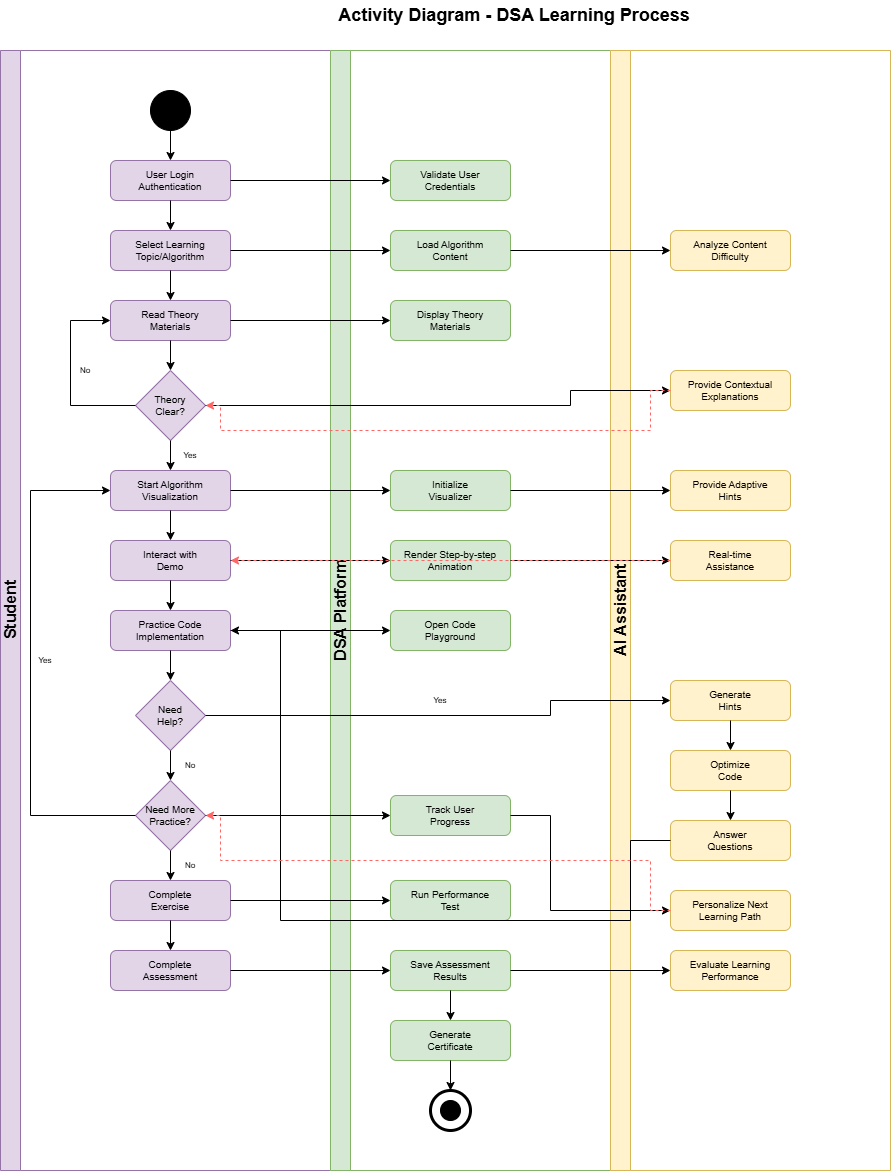
\includegraphics[width=1.0\textwidth]{enhanced-diagrams/activity-diagram-clean.png}
\caption{Activity Diagram - Main Learning Workflow}
\label{fig:activity-main-workflow}
\end{figure}

\subsection{Core Learning Process Workflow}
\label{subsec:learning-workflow}

\subsubsection{User Authentication và Authorization Flow}

\begin{enumerate}
    \item \textbf{Start}: User access application URL
    \item \textbf{Decision}: Check existing authentication status
    \item \textbf{Branch False}: Redirect to login page
    \item \textbf{Login Process}: User enters credentials (email/username + password)
    \item \textbf{Validation}: System validates credentials against database
    \item \textbf{Decision}: Credentials valid?
    \item \textbf{Branch False}: Display error message, return to login form
    \item \textbf{Branch True}: Generate JWT token, establish user session
    \item \textbf{Authorization Check}: Verify user role và permissions
    \item \textbf{Dashboard Access}: Redirect to appropriate dashboard based on role
\end{enumerate}

\subsubsection{Algorithm Learning Session Workflow}

\begin{enumerate}
    \item \textbf{Category Selection}: User browses và chọn algorithm category
    \item \textbf{Algorithm Browse}: Display available algorithms với metadata
    \item \textbf{Prerequisite Check}: Validate user có sufficient background knowledge
    \item \textbf{Decision}: Prerequisites met?
    \item \textbf{Branch False}: Suggest prerequisite algorithms hoặc background reading
    \item \textbf{Branch True}: Proceed to algorithm selection
    \item \textbf{Algorithm Selection}: User chọn specific algorithm để learn
    \item \textbf{Learning Mode Selection}: Choose between Guided, Practice, hoặc Challenge mode
    \item \textbf{Visualizer Initialization}: Load algorithm visualizer với appropriate configuration
    \item \textbf{Input Configuration}: User configure input data (custom hoặc preset examples)
    \item \textbf{Theory Study}: Optional step để review algorithm theory và concepts
    \item \textbf{Visualization Execution}: Begin interactive algorithm visualization
    \item \textbf{Step-by-step Control}: User controls animation speed, pause/resume, step forward/backward
    \item \textbf{Real-time Feedback}: System provides explanations và hints cho each step
    \item \textbf{Understanding Check}: Periodic comprehension questions during visualization
    \item \textbf{Decision}: Understanding satisfactory?
    \item \textbf{Branch False}: Provide additional explanations, repeat steps
    \item \textbf{Branch True}: Continue to completion
    \item \textbf{Session Completion}: Display final results, complexity analysis, performance metrics
    \item \textbf{Progress Update}: Update user learning progress và achievements
    \item \textbf{Recommendation Generation}: Suggest next learning objectives
\end{enumerate}

\subsubsection{AI Assistant Interaction Workflow}

\begin{enumerate}
    \item \textbf{AI Assistant Trigger}: User clicks AI help button hoặc encounters difficulty
    \item \textbf{Context Collection}: System gathers current learning context và user history
    \item \textbf{Interface Loading}: Display AI chat interface với context-aware suggestions
    \item \textbf{Query Input}: User types question hoặc selects từ suggested questions
    \item \textbf{Intent Analysis}: AI analyzes question intent và determines response strategy
    \item \textbf{Model Selection}: Choose appropriate AI model based on query type
    \item \textbf{Parallel Processing}: 
    \begin{itemize}
        \item Knowledge Retrieval từ algorithm database
        \item Context Enhancement với user learning history
        \item Response Generation với personalized explanations
    \end{itemize}
    \item \textbf{Response Formatting}: Format AI response với code highlighting, examples, links
    \item \textbf{Response Display}: Present answer với interactive elements
    \item \textbf{Follow-up Options}: Provide related questions hoặc deeper dive options
    \item \textbf{Feedback Collection}: Gather user satisfaction rating cho response quality
    \item \textbf{Conversation Continuation}: Allow follow-up questions trong same context
    \item \textbf{Session Termination}: Save conversation history, update AI interaction metrics
\end{enumerate}

\subsection{Assessment và Evaluation Workflow}
\label{subsec:assessment-workflow}

\subsubsection{Quiz Generation và Execution Process}

\begin{enumerate}
    \item \textbf{Assessment Trigger}: User completes algorithm learning hoặc explicitly requests quiz
    \item \textbf{Skill Assessment}: Analyze user current skill level và learning progress
    \item \textbf{Quiz Configuration}: Determine appropriate difficulty, question types, time limits
    \item \textbf{Dynamic Question Generation}: AI-powered question generation based on algorithm specifics
    \item \textbf{Quiz Presentation}: Display questions với appropriate interface (multiple choice, coding, interactive)
    \item \textbf{Time Management}: Track time spent per question và overall quiz duration
    \item \textbf{Answer Processing}: Validate answers real-time với immediate feedback options
    \item \textbf{Adaptive Questioning}: Adjust subsequent question difficulty based on current performance
    \item \textbf{Completion Check}: Determine khi quiz should end (all questions hoặc time limit)
    \item \textbf{Score Calculation}: Calculate final score với weighted scoring algorithm
    \item \textbf{Performance Analysis}: Analyze strong/weak areas, identify learning gaps
    \item \textbf{Recommendation Generation}: Suggest remedial learning hoặc advanced topics
    \item \textbf{Results Presentation}: Display comprehensive results với visual analytics
    \item \textbf{Progress Integration}: Integrate quiz results vào overall learning progress
\end{enumerate}

\subsection{Parallel Activities và Background Processes}
\label{subsec:parallel-activities}

\subsubsection{Real-time Analytics Collection}

Hệ thống continuously collect và process analytics data trong background:

\begin{itemize}
    \item \textbf{User Interaction Tracking}: Mouse movements, click patterns, time on sections
    \item \textbf{Learning Behavior Analysis}: Difficulty patterns, help-seeking behavior, completion rates
    \item \textbf{Performance Metrics}: Algorithm execution times, visualization rendering performance
    \item \textbf{Engagement Measurements}: Session duration, return visit patterns, feature usage
\end{itemize}

\subsubsection{System Maintenance Activities}

\begin{itemize}
    \item \textbf{Cache Management}: Periodic cache refresh và optimization
    \item \textbf{Database Optimization}: Index maintenance, query optimization
    \item \textbf{Content Updates}: Algorithm library updates, new feature deployments
    \item \textbf{Security Monitoring}: Threat detection, access pattern analysis
\end{itemize}

\section{Sequence Diagram và Interaction Analysis}
\label{sec:sequence-diagram}

\subsection{Tổng quan Sequence Modeling}
\label{subsec:sequence-overview}

Sequence Diagram được sử dụng để mô tả detailed interactions giữa các system components theo time sequence, đặc biệt focusing vào main learning scenarios và AI assistant interactions. Các diagram này illustrate message passing, object lifetimes, và coordination giữa different services.

\begin{figure}[H]
\centering
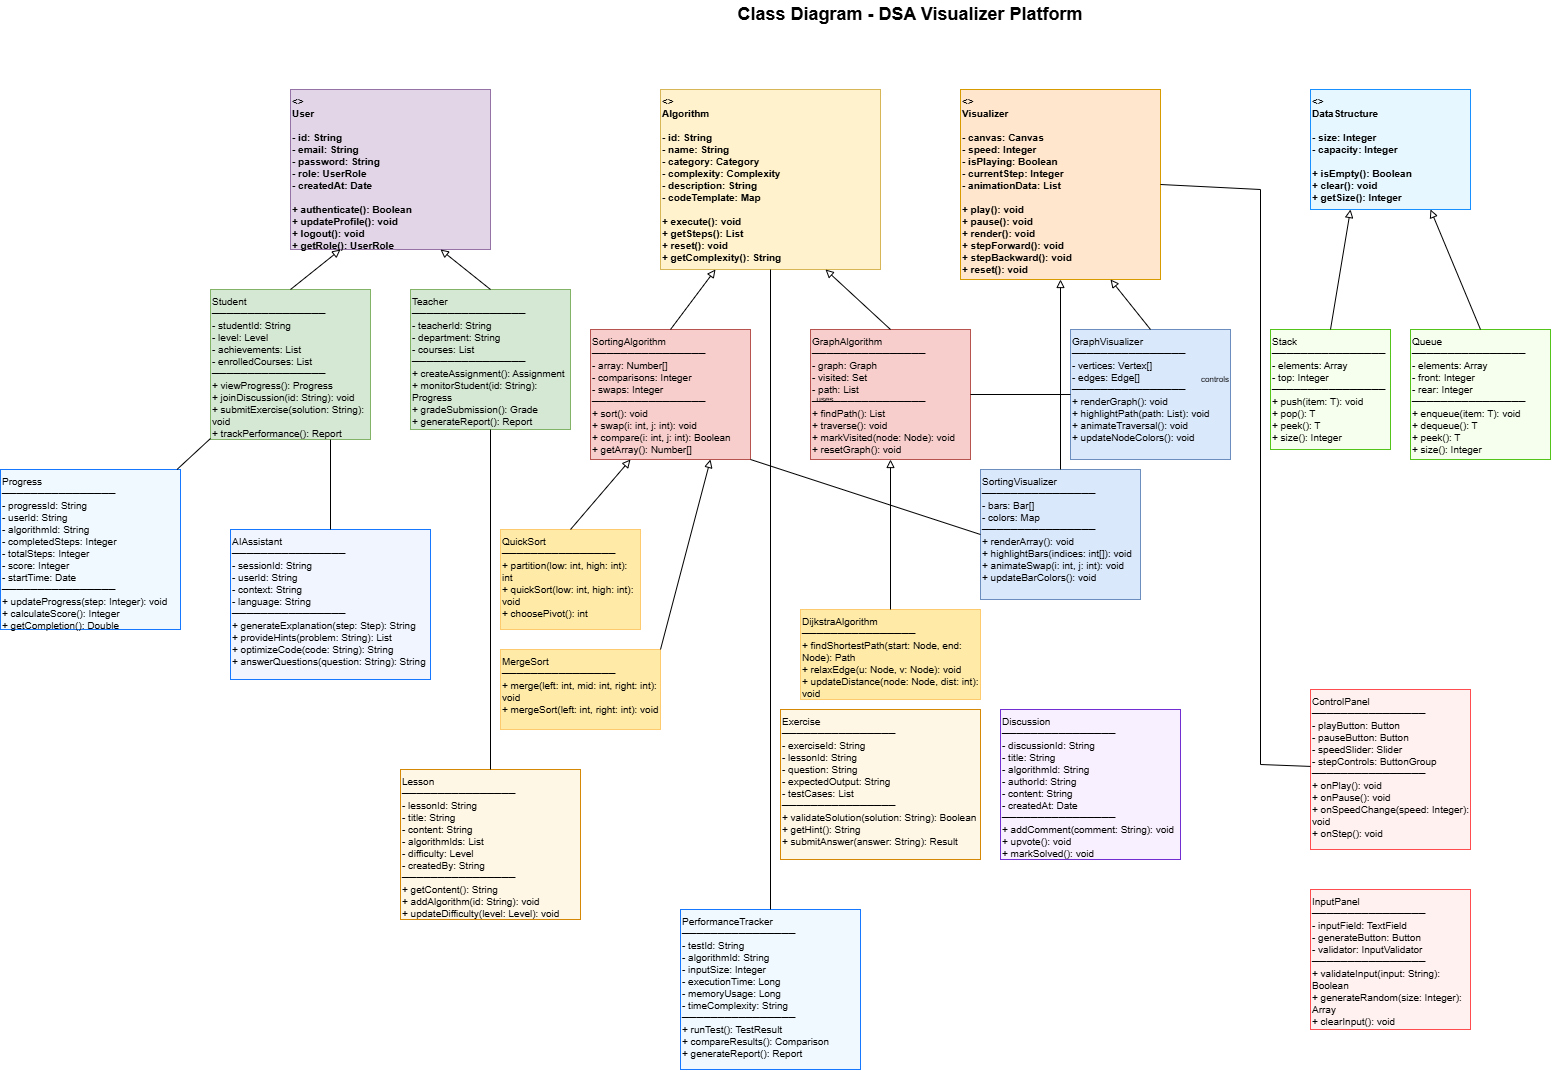
\includegraphics[width=1.0\textwidth]{enhanced-diagrams/class-diagram-clean.png}
\caption{Sequence Diagram - Algorithm Learning Process (Detailed)}
\label{fig:sequence-detailed}
\end{figure}

\subsection{Algorithm Visualization Sequence Analysis}
\label{subsec:visualization-sequence}

\subsubsection{Participants và Responsibilities}

Sequence diagram bao gồm các key participants với specific responsibilities:

\begin{itemize}
    \item \textbf{Student User}: Primary actor initiating learning activities
    \item \textbf{Browser Interface}: Frontend presentation layer handling user interactions
    \item \textbf{ReactApp Component}: Main application controller managing state và navigation
    \item \textbf{AlgorithmController Service}: Business logic layer coordinating algorithm operations
    \item \textbf{VisualizationEngine Core}: Specialized engine cho algorithm animation và rendering
    \item \textbf{AIAssistant Service}: AI-powered support service providing intelligent assistance
    \item \textbf{DataManager Repository}: Data access layer managing persistence và retrieval
    \item \textbf{Database PostgreSQL}: Storage layer containing user data, algorithms, và progress
\end{itemize}

\subsubsection{Phase 1: Initialization và Setup (Messages 1-7)}

\begin{enumerate}
    \item \textbf{Student → Browser}: selectAlgorithm(bubbleSort) - User chọn thuật toán cần học
    \item \textbf{Browser → ReactApp}: loadComponent(AlgorithmPage) - Load appropriate learning interface
    \item \textbf{ReactApp → AlgorithmController}: initializeAlgorithm(bubbleSort) - Setup algorithm context
    \item \textbf{AlgorithmController → VisualizationEngine}: createVisualization(config) - Initialize visualization environment
    \item \textbf{VisualizationEngine → AIAssistant}: getExplanation(algorithm) - Request contextual explanations
    \item \textbf{AIAssistant → DataManager}: fetchAlgorithmData() - Retrieve algorithm metadata và examples
    \item \textbf{DataManager → Database}: SELECT * FROM algorithms - Database query cho algorithm details
\end{enumerate}

\textbf{Return Flow}: Database returns algorithm details → DataManager processes data → AIAssistant generates explanations → VisualizationEngine prepares rendering → AlgorithmController confirms setup → ReactApp loads interface → Browser displays algorithm page → Student receives interactive learning environment.

\subsubsection{Phase 2: Data Input và Execution Setup (Messages 8-12)}

\begin{enumerate}
    \item \textbf{Student → Browser}: inputData([64,34,25,12,22]) - User provides input data for algorithm
    \item \textbf{Browser → ReactApp}: setArrayData(data) - Frontend processes và validates input
    \item \textbf{Student → Browser}: startSorting() - User initiates algorithm execution
    \item \textbf{Browser → ReactApp}: executeAlgorithm() - Trigger algorithm execution workflow
    \item \textbf{ReactApp → AlgorithmController}: runBubbleSort(array) - Start specific algorithm với input data
\end{enumerate}

\subsubsection{Phase 3: Algorithm Processing với Loop Fragment (Messages 13-16)}

Loop fragment được implement để handle iterative algorithm execution:

\textbf{Loop Condition}: [for each step in algorithm execution]

\begin{enumerate}
    \item \textbf{AlgorithmController → VisualizationEngine}: animateStep(step) - Animate current algorithm step
    \item \textbf{VisualizationEngine → ReactApp}: updateVisualization() - Update UI với current state
    \item \textbf{ReactApp → Browser}: renderStep() - Render animation frame
    \item \textbf{Browser → Student}: displayStep() - Show visual representation to user
\end{enumerate}

\textbf{Loop Continuation}: Process repeats until algorithm completion, với user có ability để pause, resume, hoặc adjust speed.

\subsubsection{Final Return Messages}

Khi algorithm execution complete:
\begin{itemize}
    \item VisualizationEngine signals completion
    \item AlgorithmController processes final results
    \item ReactApp updates completion status
    \item Browser displays final sorted array và performance metrics
    \item Student receives completion confirmation với learning analytics
\end{itemize}

\subsection{AI Assistant Interaction Sequence}
\label{subsec:ai-interaction-sequence}

\subsubsection{Multi-Model AI Architecture}

Hệ thống implements sophisticated AI architecture với multiple models:

\begin{enumerate}
    \item \textbf{Context Router}: Intelligent routing based on query type và complexity
    \item \textbf{OpenAI GPT Integration}: Specialized cho natural language explanations và conceptual questions
    \item \textbf{Google Gemini Integration}: Optimized cho code generation, analysis, và technical details
    \item \textbf{Response Aggregator}: Combines insights từ multiple models when appropriate
\end{enumerate}

\subsubsection{AI Assistance Sequence Flow}

\begin{enumerate}
    \item \textbf{Context Collection}: AIAssistant gathers current learning context, user history, và algorithm state
    \item \textbf{Intent Analysis}: Natural language processing để understand user question intent
    \item \textbf{Model Selection}: Intelligent routing đến appropriate AI model based on query characteristics
    \item \textbf{Knowledge Retrieval}: Access relevant algorithm documentation, examples, và best practices
    \item \textbf{Response Generation}: Generate contextual, personalized response với code examples
    \item \textbf{Quality Assurance}: Validate response accuracy và appropriateness cho user level
    \item \textbf{Response Delivery}: Format và present response với rich formatting, syntax highlighting
    \item \textbf{Feedback Loop}: Collect user satisfaction để improve future responses
\end{enumerate}

\subsection{Error Handling và Recovery Sequences}
\label{subsec:error-handling-sequences}

\subsubsection{Service Unavailable Recovery}

Khi AI service hoặc other critical services become unavailable:

\begin{enumerate}
    \item \textbf{Service Monitor}: Detects service failure hoặc timeout
    \item \textbf{Fallback Activation}: Automatically switch to backup resources
    \item \textbf{User Notification}: Inform user về temporary limitations
    \item \textbf{Graceful Degradation}: Provide alternative functionality
    \item \textbf{Service Recovery}: Monitor và restore service khi available
    \item \textbf{Resume Normal Operation}: Seamlessly return to full functionality
\end{enumerate}

\subsubsection{Data Validation và Input Error Handling}

\begin{enumerate}
    \item \textbf{Input Validation}: Real-time validation của user input data
    \item \textbf{Error Detection}: Identify specific validation failures
    \item \textbf{User Feedback}: Provide clear, actionable error messages
    \item \textbf{Correction Guidance}: Suggest valid input formats và examples
    \item \textbf{Auto-correction}: Offer to automatically fix common input errors
    \item \textbf{Retry Mechanism}: Allow user to retry với corrected input
\end{enumerate}

\section{System Architecture và Technical Design}
\label{sec:system-architecture}

\subsection{Architectural Overview}
\label{subsec:architecture-overview}

Hệ thống DSA Visualizer được thiết kế theo Multi-Layer Architecture pattern với clear separation of concerns, ensuring scalability, maintainability, và performance optimization. Architecture được organize thành 5 distinct layers, mỗi layer có specific responsibilities và well-defined interfaces.

\begin{figure}[H]
\centering
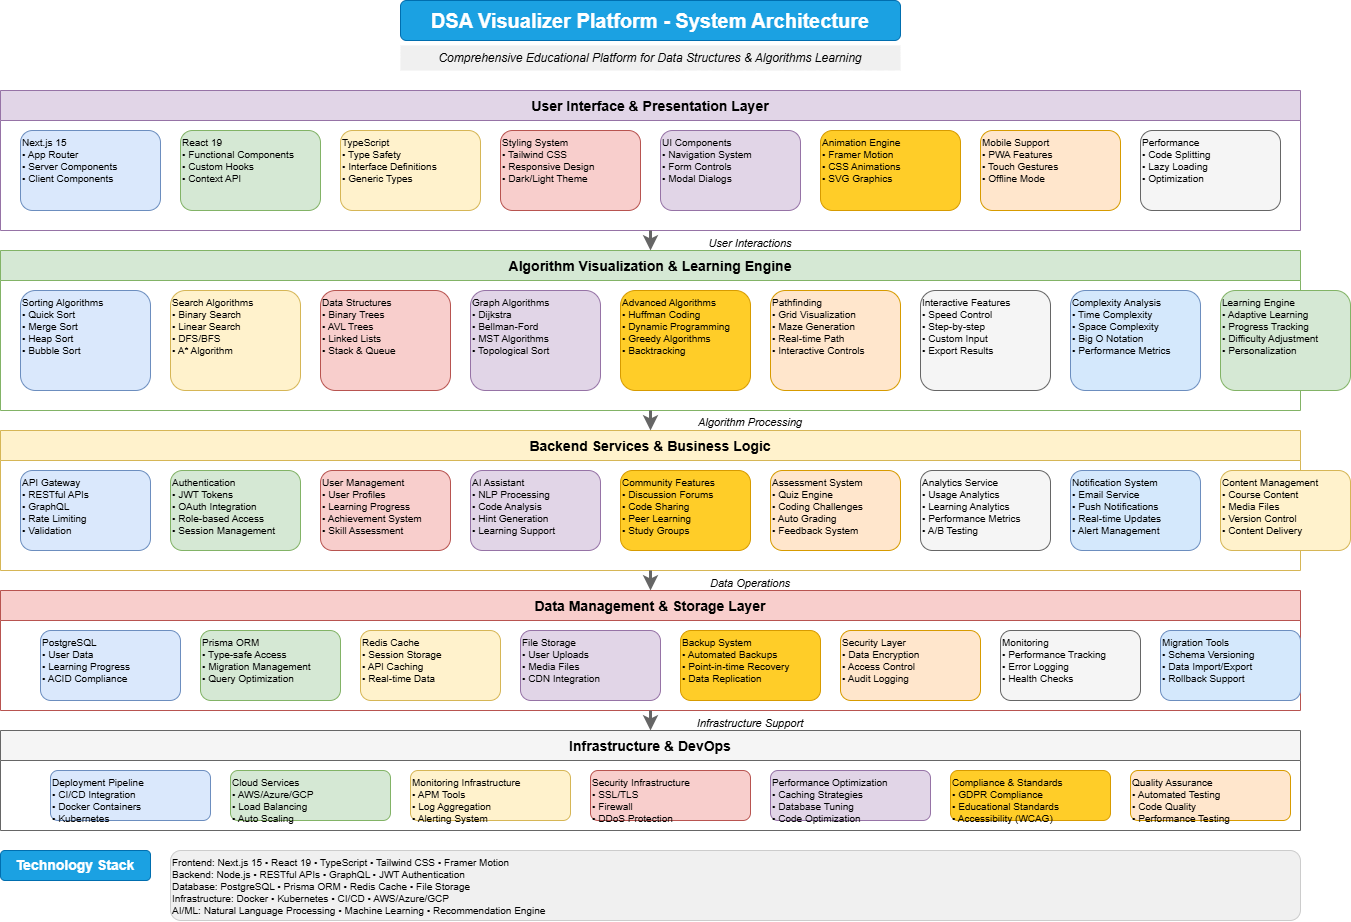
\includegraphics[width=1.0\textwidth]{enhanced-diagrams/system-architecture-clean.png}
\caption{System Architecture - Multi-Layer Design}
\label{fig:system-architecture}
\end{figure}

\subsection{Layer-by-Layer Analysis}
\label{subsec:layer-analysis}

\subsubsection{Layer 1: Presentation Layer (UI/Frontend)}

\textbf{Technologies}: Next.js 14, React 18, TypeScript, TailwindCSS, Framer Motion

\textbf{Core Components}:
\begin{itemize}
    \item \textbf{Interactive Visualizers}: Canvas-based algorithm animations với real-time rendering
    \item \textbf{Control Interfaces}: Speed control, step navigation, pause/resume functionality
    \item \textbf{Dashboard Systems}: User progress tracking, analytics visualization, achievement displays
    \item \textbf{AI Chat Interface}: Real-time conversational AI với context-aware responses
    \item \textbf{Assessment Platform}: Interactive quizzes, coding challenges, instant feedback systems
\end{itemize}

\textbf{Design Patterns Implemented}:
\begin{itemize}
    \item Component-based architecture với reusable UI elements
    \item State management using React Context API và custom hooks
    \item Responsive design patterns cho mobile-first approach
    \item Progressive Web App (PWA) features cho offline capability
\end{itemize}

\subsubsection{Layer 2: Visualization Engine Layer}

\textbf{Technologies}: D3.js, HTML5 Canvas API, WebGL, Three.js

\textbf{Core Subsystems}:
\begin{itemize}
    \item \textbf{Animation Controller}: Manages complex animation timelines, keyframe interpolation, easing functions
    \item \textbf{Rendering Engine}: High-performance visualization rendering với GPU acceleration
    \item \textbf{Interaction Handler}: Processes user interactions với visualizations (drag, zoom, selection)
    \item \textbf{State Manager}: Tracks algorithm execution state, enables undo/redo functionality
    \item \textbf{Performance Monitor}: Real-time performance tracking và optimization
\end{itemize}

\textbf{Visualization Capabilities}:
\begin{itemize}
    \item Dynamic array/list visualizations với color-coded elements
    \item Interactive tree structures với expandable/collapsible nodes
    \item Graph visualizations với animated edge traversal
    \item Multi-algorithm comparison views với synchronized playback
    \item 3D visualizations cho complex data structures
\end{itemize}

\subsubsection{Layer 3: Backend Services Layer}

\textbf{Technologies}: Node.js, Express.js, TypeScript, Microservices Architecture

\textbf{Microservices Portfolio}:
\begin{itemize}
    \item \textbf{Algorithm Service}: Algorithm execution engine, step generation, complexity analysis
    \item \textbf{User Management Service}: Authentication, authorization, profile management, role-based access control
    \item \textbf{Learning Service}: Progress tracking, session management, learning path optimization
    \item \textbf{Assessment Service}: Quiz generation, automated scoring, performance analytics
    \item \textbf{AI Integration Service}: Multi-model AI coordination, context management, response optimization
    \item \textbf{Analytics Service}: User behavior tracking, learning analytics, predictive modeling
    \item \textbf{Notification Service}: Real-time notifications, email alerts, achievement announcements
\end{itemize}

\textbf{API Design Principles}:
\begin{itemize}
    \item RESTful APIs với comprehensive OpenAPI documentation
    \item GraphQL endpoints cho complex data relationships
    \item WebSocket connections cho real-time features
    \item Rate limiting, request throttling, security middleware
    \item API versioning strategy cho backward compatibility
\end{itemize}

\subsubsection{Layer 4: Data Management Layer}

\textbf{Technologies}: MongoDB, PostgreSQL, Redis, Elasticsearch

\textbf{Database Strategy}:
\begin{itemize}
    \item \textbf{MongoDB}: User profiles, learning sessions, unstructured content, algorithm metadata
    \item \textbf{PostgreSQL}: Structured data, relational analytics, reporting, audit logs
    \item \textbf{Redis}: Session caching, real-time leaderboards, temporary data storage
    \item \textbf{Elasticsearch}: Full-text search, content discovery, advanced analytics
\end{itemize}

\textbf{Data Models và Relationships}:
\begin{itemize}
    \item Normalized user entities với comprehensive profile management
    \item Algorithm catalog với versioning và metadata management
    \item Learning progress tracking với detailed analytics
    \item Assessment results với statistical analysis capabilities
    \item Content management với multilingual support
\end{itemize}

\subsubsection{Layer 5: Infrastructure Layer}

\textbf{Deployment Strategy}: Container-based deployment với Kubernetes orchestration

\textbf{Cloud Infrastructure}:
\begin{itemize}
    \item \textbf{Compute Resources}: Auto-scaling web servers, load balancers, container clusters
    \item \textbf{Storage Solutions}: Distributed file storage, CDN integration, backup systems
    \item \textbf{Security}: WAF protection, DDoS mitigation, SSL/TLS encryption
    \item \textbf{Monitoring}: Application performance monitoring, log aggregation, alerting systems
\end{itemize}

\textbf{DevOps Pipeline}:
\begin{itemize}
    \item Continuous Integration/Continuous Deployment (CI/CD) với automated testing
    \item Infrastructure as Code (IaC) sử dụng Terraform
    \item Monitoring và logging với Prometheus, Grafana, ELK stack
    \item Security scanning với SAST/DAST tools
\end{itemize}

\subsection{Integration Patterns và Communication}
\label{subsec:integration-patterns}

\subsubsection{Event-Driven Architecture}

Hệ thống implements comprehensive event-driven patterns:

\begin{itemize}
    \item \textbf{User Interaction Events}: UI events trigger visualization updates, progress tracking
    \item \textbf{Learning Progress Events}: Automatic progress updates, achievement unlocking
    \item \textbf{System Health Events}: Performance monitoring, error detection, alerting
    \item \textbf{AI Interaction Events}: Context updates, model optimization, feedback collection
\end{itemize}

\subsubsection{Caching Strategy}

Multi-level caching approach cho optimal performance:

\begin{itemize}
    \item \textbf{Browser Caching}: Static assets, compiled code, user preferences
    \item \textbf{CDN Caching}: Global content distribution, image optimization
    \item \textbf{Application Caching}: Frequently accessed data, computed results
    \item \textbf{Database Caching}: Query result caching, connection pooling
\end{itemize}

\subsubsection{Security Architecture}

Comprehensive security measures implemented across all layers:

\begin{itemize}
    \item \textbf{Authentication}: JWT-based authentication với refresh token rotation
    \item \textbf{Authorization}: Role-based access control (RBAC) với fine-grained permissions
    \item \textbf{Data Protection}: Encryption at rest và in transit, PII anonymization
    \item \textbf{Input Validation}: Comprehensive input sanitization, XSS/CSRF protection
    \item \textbf{API Security}: Rate limiting, API key management, request validation
\end{itemize}

\section{Performance Optimization và Quality Assurance}
\label{sec:performance-quality}

\subsection{Performance Optimization Strategies}
\label{subsec:performance-optimization}

\subsubsection{Frontend Performance}

\begin{itemize}
    \item \textbf{Code Splitting}: Dynamic imports, route-based splitting, component-level lazy loading
    \item \textbf{Bundle Optimization}: Tree shaking, dead code elimination, compression algorithms
    \item \textbf{Rendering Optimization}: Virtual DOM optimization, memoization, efficient re-rendering
    \item \textbf{Asset Optimization}: Image compression, WebP format, progressive loading
    \item \textbf{Memory Management}: Efficient data structures, garbage collection optimization
\end{itemize}

\subsubsection{Backend Performance}

\begin{itemize}
    \item \textbf{Database Optimization}: Query optimization, proper indexing strategies, connection pooling
    \item \textbf{Caching Implementation}: Multi-level caching, cache invalidation strategies
    \item \textbf{Asynchronous Processing}: Non-blocking I/O, worker threads, background job processing
    \item \textbf{Load Balancing}: Horizontal scaling, session affinity, health check monitoring
    \item \textbf{Resource Management}: Memory optimization, CPU utilization monitoring
\end{itemize}

\subsection{Quality Assurance Framework}
\label{subsec:quality-assurance}

\subsubsection{Testing Strategy}

\begin{itemize}
    \item \textbf{Unit Testing}: Component testing, service testing, utility function testing
    \item \textbf{Integration Testing}: API testing, database integration, service communication
    \item \textbf{End-to-End Testing}: User journey testing, cross-browser compatibility
    \item \textbf{Performance Testing}: Load testing, stress testing, scalability testing
    \item \textbf{Security Testing}: Penetration testing, vulnerability scanning, security audits
\end{itemize}

\subsubsection{Code Quality Standards}

\begin{itemize}
    \item \textbf{Code Style}: ESLint, Prettier, TypeScript strict mode
    \item \textbf{Code Review}: Pull request reviews, automated code analysis
    \item \textbf{Documentation}: Comprehensive API documentation, inline code comments
    \item \textbf{Version Control}: Git best practices, semantic versioning, branching strategy
\end{itemize}

\section{Kết luận Chapter 3}
\label{sec:chapter3-conclusion}

Chapter 3 đã cung cấp comprehensive analysis của hệ thống DSA Visualizer từ multiple perspectives, establishing solid foundation cho implementation phase. Các achievements chính bao gồm:

\subsection{Use Case Analysis Completion}

Đã định nghĩa và documented chi tiết 5 core use cases với full specification tables:
\begin{itemize}
    \item UC001: Algorithm Visualization Learning - Core learning functionality
    \item UC002: Interactive Algorithm Practice - Hands-on practice environment
    \item UC003: AI Assistant Consultation - Intelligent learning support
    \item UC004: Algorithm Comparison Analysis - Comparative learning tools
    \item UC005: Learning Progress Tracking - Progress monitoring và analytics
\end{itemize}

\subsection{UML Modeling Excellence}

\begin{itemize}
    \item \textbf{Class Diagram}: Comprehensive OOP design với design patterns implementation
    \item \textbf{Activity Diagram}: Detailed workflow analysis với decision points và parallel activities
    \item \textbf{Sequence Diagram}: In-depth interaction analysis với timing và message flows
\end{itemize}

\subsection{Architectural Design}

Established robust 5-layer architecture ensuring:
\begin{itemize}
    \item \textbf{Scalability}: Microservices design cho independent scaling
    \item \textbf{Maintainability}: Clean architecture với clear separation of concerns
    \item \textbf{Performance}: Multi-level optimization strategies
    \item \textbf{Security}: Comprehensive security measures across all layers
\end{itemize}

\subsection{Technical Excellence}

Applied industry best practices:
\begin{itemize}
    \item SOLID principles implementation
    \item Design patterns cho reusability và flexibility
    \item Performance optimization strategies
    \item Quality assurance frameworks
\end{itemize}

Với foundation được establish trong Chapter 3, Chapter 4 sẽ focus vào detailed implementation specifications, technical architecture details, và deployment strategies cho successful system realization.
